\section{Global Use Case Analysis}

The global use case diagram provides a comprehensive overview of the Credix payment system's functional scope, illustrating the complete interaction landscape between system actors and their respective capabilities. This diagram serves as the foundational blueprint for understanding the system's behavioral requirements and sprint organization.

\subsection{System Actors and Responsibilities}

The Credix ecosystem operates through two primary actors, each with distinct roles and access privileges:

\textbf{Corporate Actor:} Represents the business entities that utilize Credix for employee payment management. This actor encompasses the administrative and managerial functions essential for organizational payment operations, including bulk credit management, user administration, financial oversight, and comprehensive analytics capabilities.

\textbf{End User Actor:} Represents individual employees or beneficiaries who utilize the Credix mobile application for daily payment transactions. This actor focuses on transactional capabilities, account management, and real-time payment processing functionalities.

\subsection{Use Case Organization and Sprint Mapping}

The global use case diagram strategically organizes system functionality across four development sprints, with each sprint addressing specific business priorities and technical complexities:

\begin{figure}[H]
    \centering
    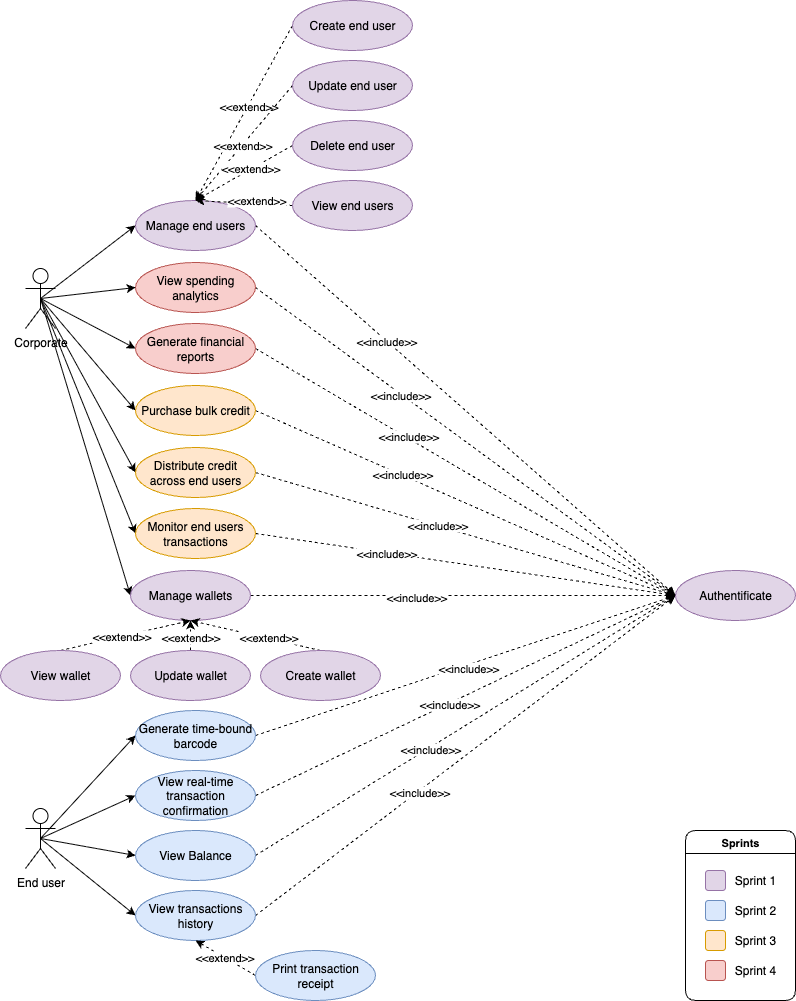
\includegraphics[width=0.9\textwidth]{images/usecase_global.png}
    \caption{Global Use Case Diagram - Complete System Overview}
    \label{fig:global_usecase}
\end{figure}

\textbf{Sprint 1 (Purple):} Establishes foundational user management capabilities, enabling Corporate actors to create, update, delete, and view end users within the system. This sprint includes comprehensive wallet management functionality, providing the administrative foundation necessary for subsequent payment operations.

\textbf{Sprint 2 (Blue):} Implements core end-user transactional capabilities, including balance viewing, transaction history access, time-bound barcode generation for secure payments, and real-time transaction confirmation systems. This sprint delivers the essential payment functionality that end users require for daily operations.

\textbf{Sprint 3 (Orange):} Focuses on advanced credit management operations, enabling Corporate actors to purchase bulk credit, distribute credit across end users, and monitor end user transactions. This sprint addresses the sophisticated financial management requirements of corporate clients.

\textbf{Sprint 4 (Red):} Delivers comprehensive analytics and reporting capabilities, allowing Corporate actors to view spending analytics and generate detailed financial reports. This sprint provides the business intelligence tools necessary for informed decision-making and financial oversight.

\subsection{Cross-Cutting Concerns}

The diagram illustrates several critical cross-cutting concerns that span multiple use cases:

\textbf{Authentication:} Every use case includes authentication requirements, ensuring secure access control throughout the system. This universal security requirement demonstrates the system's commitment to financial data protection and regulatory compliance.

\textbf{Extend Relationships:} Multiple use cases utilize extend relationships to provide specialized functionality while maintaining core use case simplicity. For example, user management extends to specific CRUD operations, and transaction viewing extends to receipt printing capabilities.

\textbf{Include Relationships:} The extensive use of include relationships with authentication demonstrates the system's security-first approach, ensuring that all functional capabilities require proper user verification before execution.

This global use case analysis provides the architectural foundation for detailed sprint planning and implementation, ensuring comprehensive coverage of business requirements while maintaining clear separation of concerns across different user roles and system capabilities.
